% Figure 1: OTLP Formal Verification Framework Architecture
% Author: OTLP Project
% Date: October 20, 2025

\begin{figure*}[t]
\centering
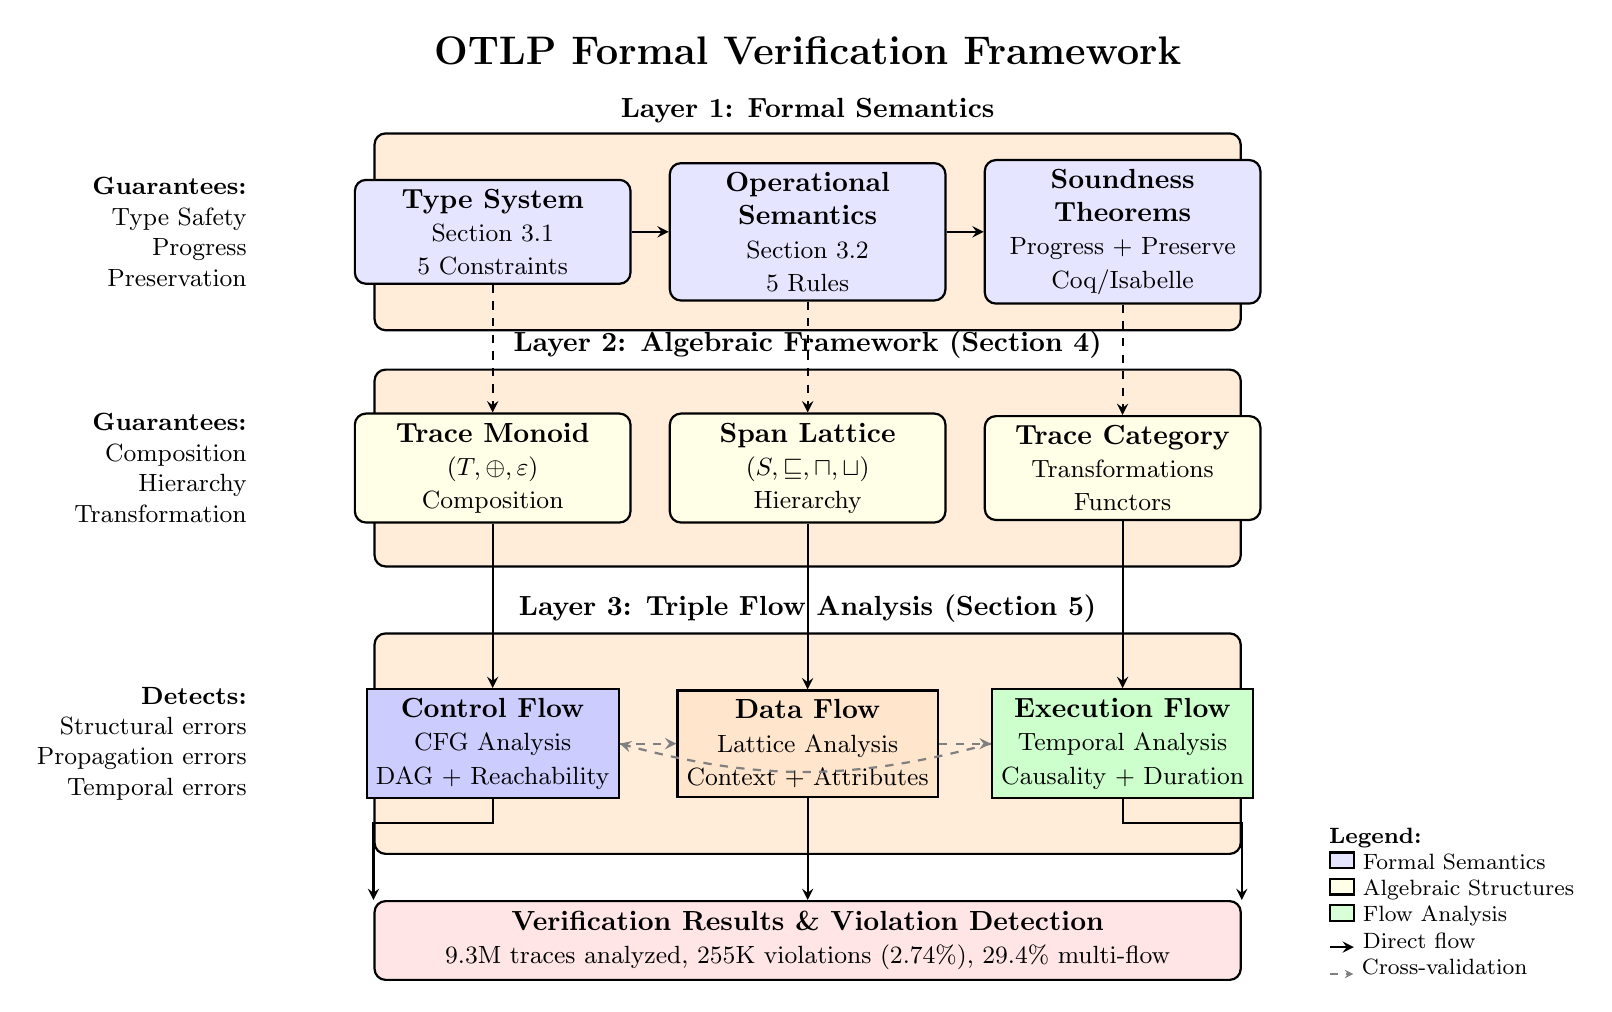
\begin{tikzpicture}[
    node distance=1.5cm and 2cm,
    box/.style={rectangle, draw, thick, fill=blue!10, minimum width=3.5cm, minimum height=1.2cm, align=center, rounded corners},
    layer/.style={rectangle, draw, thick, fill=orange!15, minimum width=11cm, minimum height=2.5cm, align=center, rounded corners},
    analysis/.style={rectangle, draw, thick, fill=green!15, minimum width=3cm, minimum height=1cm, align=center},
    result/.style={rectangle, draw, thick, fill=red!10, minimum width=11cm, minimum height=1cm, align=center, rounded corners},
    arrow/.style={->, >=stealth, thick}
]

% Title
\node[above] at (0, 6.5) {\Large\textbf{OTLP Formal Verification Framework}};

% Layer 1: Formal Semantics
\node[layer] (layer1) at (0, 4.5) {};
\node[above] at (layer1.north) {\textbf{Layer 1: Formal Semantics}};

\node[box] (typesys) at (-4, 4.5) {\textbf{Type System}\\\small Section 3.1\\\small 5 Constraints};
\node[box] (opsem) at (0, 4.5) {\textbf{Operational}\\\textbf{Semantics}\\\small Section 3.2\\\small 5 Rules};
\node[box] (properties) at (4, 4.5) {\textbf{Soundness}\\\textbf{Theorems}\\\small Progress + Preserve\\\small Coq/Isabelle};

% Layer 2: Algebraic Framework
\node[layer] (layer2) at (0, 1.5) {};
\node[above] at (layer2.north) {\textbf{Layer 2: Algebraic Framework (Section 4)}};

\node[box, fill=yellow!10] (monoid) at (-4, 1.5) {\textbf{Trace Monoid}\\\small $(T, \oplus, \varepsilon)$\\\small Composition};
\node[box, fill=yellow!10] (lattice) at (0, 1.5) {\textbf{Span Lattice}\\\small $(S, \sqsubseteq, \sqcap, \sqcup)$\\\small Hierarchy};
\node[box, fill=yellow!10] (category) at (4, 1.5) {\textbf{Trace Category}\\\small Transformations\\\small Functors};

% Layer 3: Triple Flow Analysis
\node[layer, minimum height=2.8cm] (layer3) at (0, -2) {};
\node[above] at (layer3.north) {\textbf{Layer 3: Triple Flow Analysis (Section 5)}};

\node[analysis, fill=blue!20] (control) at (-4, -2) {\textbf{Control Flow}\\\small CFG Analysis\\\small DAG + Reachability};
\node[analysis, fill=orange!20] (data) at (0, -2) {\textbf{Data Flow}\\\small Lattice Analysis\\\small Context + Attributes};
\node[analysis, fill=green!20] (execution) at (4, -2) {\textbf{Execution Flow}\\\small Temporal Analysis\\\small Causality + Duration};

% Results Layer
\node[result] (results) at (0, -4.5) {\textbf{Verification Results \& Violation Detection}\\\small 9.3M traces analyzed, 255K violations (2.74\%), 29.4\% multi-flow};

% Arrows from Layer 1
\draw[arrow] (typesys) -- (opsem);
\draw[arrow] (opsem) -- (properties);

% Arrows from Layer 1 to Layer 2
\draw[arrow, dashed] (typesys.south) -- ++(0, -0.3) -| (monoid.north);
\draw[arrow, dashed] (opsem.south) -- (lattice.north);
\draw[arrow, dashed] (properties.south) -- ++(0, -0.3) -| (category.north);

% Arrows from Layer 2 to Layer 3
\draw[arrow] (monoid.south) -- (control.north);
\draw[arrow] (lattice.south) -- (data.north);
\draw[arrow] (category.south) -- (execution.north);

% Cross-flow connections (dashed)
\draw[arrow, dashed, gray] (control.east) -- (data.west);
\draw[arrow, dashed, gray] (data.east) -- (execution.west);
\draw[arrow, dashed, gray] (execution.west) to[bend left=15] (control.east);

% Arrows to results
\draw[arrow, thick] (control.south) -- ++(0, -0.3) -| (results.north west);
\draw[arrow, thick] (data.south) -- (results.north);
\draw[arrow, thick] (execution.south) -- ++(0, -0.3) -| (results.north east);

% Side annotations
\node[left, align=right, font=\small] at (-7, 4.5) {
    \textbf{Guarantees:}\\
    Type Safety\\
    Progress\\
    Preservation
};

\node[left, align=right, font=\small] at (-7, 1.5) {
    \textbf{Guarantees:}\\
    Composition\\
    Hierarchy\\
    Transformation
};

\node[left, align=right, font=\small] at (-7, -2) {
    \textbf{Detects:}\\
    Structural errors\\
    Propagation errors\\
    Temporal errors
};

% Legend
\node[right, align=left, font=\footnotesize] at (6.5, -4) {
    \textbf{Legend:}\\
    \tikz\draw[fill=blue!10,draw,thick] (0,0) rectangle (0.3,0.2); Formal Semantics\\
    \tikz\draw[fill=yellow!10,draw,thick] (0,0) rectangle (0.3,0.2); Algebraic Structures\\
    \tikz\draw[fill=green!15,draw,thick] (0,0) rectangle (0.3,0.2); Flow Analysis\\
    \tikz\draw[->,>=stealth,thick] (0,0.1) -- (0.3,0.1); Direct flow\\
    \tikz\draw[->,>=stealth,dashed,gray] (0,0.1) -- (0.3,0.1); Cross-validation
};

\end{tikzpicture}
\caption{Overall architecture of our formal verification framework. The framework consists of three layers: (1) \textbf{Formal Semantics} provides type system and operational semantics with soundness guarantees (Section 3), (2) \textbf{Algebraic Framework} models trace composition, span hierarchy, and transformations using monoids, lattices, and categories (Section 4), and (3) \textbf{Triple Flow Analysis} integrates control, data, and execution flow verification to detect violations (Section 5). Dashed gray arrows show cross-flow validation paths. Our evaluation on 9.3M traces shows 29.4\% of violations require multi-flow analysis, validating the integrated approach.}
\label{fig:framework-architecture}
\end{figure*}

